\documentclass[12pt]{article}

\usepackage{a4wide, amsfonts, epsfig}

\begin{document}
\begin{center}
{\bf EMAT10001 Workshop Sheet 17.}\\[1cm]{} Conor Houghton 2014-02-26
\end{center}
\subsubsection*{Introduction} 
This worksheet is about Fourier series. There is the usual bounty for errors and typos, 20p to \pounds
2 depending on how serious it is.

\subsubsection*{Useful facts}
\begin{itemize}

\item {\bf Trigonometric identities}: adding angles
\begin{eqnarray}
\sin{A\pm B}&=&\sin{A}\cos{B}\pm\cos{A}\sin{B}\cr
\cos{A\pm B}&=&\cos{A}\cos{B}\mp\sin{A}\sin{B}.
\end{eqnarray}
\item {\bf Trigonometric identities}: products
\begin{eqnarray}
\cos{A}\cos{B}&=&\frac{1}{2}[\cos{(A-B)}+\cos{(A+B)}]\cr
\sin{A}\sin{B}&=&\frac{1}{2}[\cos{(A-B)}-\cos{(A+B)}]\cr
\sin{A}\cos{B}&=&\frac{1}{2}[\sin{(A+B)}+\sin{(A-B)}].
\end{eqnarray}
\item {\bf Trigonometric identities}: double angles
\begin{eqnarray}
\sin{2A}&=&2\sin{A}\cos{A}\cr
\cos{2A}&=&\cos^2{A}-\sin^2{A}.
\end{eqnarray}

\item The integral of a sine or a cosine over its whole period is
  zero, the negative and positive balance.

\item {\bf The Kronecker delta}: $\delta_{nm}$ is zero when $n\not=m$ and one when $n=m$.

\item {\bf Periodic}: A function is periodic if for some constant $L$, $f(t+L)=f(t)$. The smallest such $L$ is called the {\sl period}.

\item {\bf Periodic, even and odd} A function $f(t)$ has period $L$ if $f(t+L)=f(t)$, it is odd if
$f(-t)=-f(t)$ and even if $f(-t)=f(t)$.

\item A function with period $L$ has the {\bf Fourier series expansion}
$$f(t)={a_0\over2}+\sum_{n=1}^\infty ~a_n \cos\left({2\pi n t\over L}\right)+\sum_{n=1}^\infty ~b_n \sin\left({2\pi n t\over L}\right).$$
where 
\begin{eqnarray*}
a_0&=&\frac{2}{L}\int_{-L/2}^{L/2}f(t)dt\cr
a_n&=&\frac{2}{L}\int_{-L/2}^{L/2}f(t) \cos\left({2\pi n t\over L}\right) dt\cr
b_n&=&\frac{2}{L}\int_{-L/2}^{L/2}f(t) \sin\left({2\pi n t\over L}\right) dt
\end{eqnarray*}


\item In the lectures we considered only $L=2\pi$:
$$f(t)={a_0\over2}+\sum_{n=1}^\infty ~a_n \cos(n t)+\sum_{n=1}^\infty ~b_n \sin(n t).$$
where 
\begin{eqnarray*}
a_0&=&\frac{1}{\pi}\int_{-\pi}^{\pi}f(t)dt\cr
a_n&=&\frac{1}{\pi}\int_{-\pi}^{\pi}f(t) \cos(n t) dt\cr
b_n&=&\frac{1}{\pi}\int_{-\pi}^{\pi}f(t) \sin(n t) dt
\end{eqnarray*}

\end{itemize}
\subsubsection*{Work sheet}

\begin{enumerate}

\item Establish that
\begin{equation}
\int^\pi_{-\pi}~ \sin mt ~\cos nt dt=0
\end{equation}
for integers $n$ and $m$.

\item What is $\sum_{n=0}^\infty a_n\delta_{n3}$?

\item Show by checking whether $f(t)=-f(-t)$ for odd, $f(t)=f(-t)$ for even and neither for neither which of the following are odd, even or neither: $\sin{t}$, $t^3+t$, $t^3+2t^2$ and $|t|$.

\item Consider an odd function $f(t)$. By doing a change of variable
  $t'=-t$ show 
 \begin{equation}
\int_{-1}^1f(t)dt=0
\end{equation}

\item If $f(t)$ is even and $g(t)$ is odd, what is $f(t)g(t)$?

\item What is the Fourier series for 
\begin{equation}
f(t)=\left\{\begin{array}{ll}-1&t\in(-\pi,-\pi/2)\\
                             1 &t\in(-\pi/2,\pi/2)\\
                             -1&t\in(\pi/2,\pi)
\end{array}\right.
\end{equation}
with $f(t+2\pi)=f(t)$. Try to use odd and even arguments to avoid
doing the integral for $b_n$.

\item There are, roughly speaking, two different types of sleep, slow
  wave sleep (SWS) when the brain is largely in active and the body is
  relaxed, and rapid eye movement (REM) sleep when we dream, the brain
  has a similar activity pattern to waking and the body is
  paralysed. This was discovered using electroencephalogram (EEG), the
  recording of the electrical activity in the brain using electrodes
  placed on the scalp. Here we see, on the left, EEG traces for a
  mouse during REM, SWS and waking, on the right we see a measure of
  the size of the Fourier components, roughly the $a_n$ and $b_n$ for
  different frequencies: $\sin(n t)$ has period $2\pi/n$ and so has
  frequency $n/2\pi$. Although the brain is largely inactive during
  SWS what little activity there is is synchronized and is
  characterized by delta waves and theta waves. Can you guess what
  frequency delta waves and theta waves are at? [Picture taken from Lima SL, Rattenborg NC, Lesku JA, Amlaner CJ. (2005) \textsl{Sleeping under the risk of predation.} Animal Behaviour 70:723-736.]  
\begin{center}
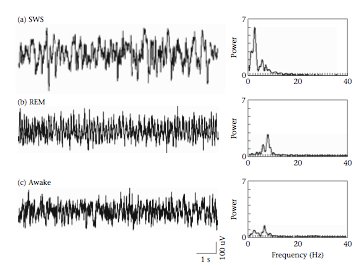
\includegraphics{SleepGeneral.png}
\end{center}
\end{enumerate}


\subsubsection*{Exercise sheet}

The difference between the work sheet and the exercise sheet is that
the solutions to the exercise sheet won't be given and the problems
are designed to be more suited to working on on your own, though you
are free to discuss them in the work shop if you finish the work sheet
problems. Selected problems from the exercise sheet will be requested
as part of the continual assessment portfolio.

\begin{enumerate}


\item Establish that
\begin{equation}
\frac{1}{\pi}\int^\pi_{-\pi} \cos mt ~\cos nt dt=\delta_{mn}
\end{equation}
for integers $n$ and $m$.

\item Read the wikipedia page for the Fast Fourier Transform.

\item Using \texttt{gnuplot} or whatever plot the function, written here in a Fourier series form
\begin{equation}
f(t)=\sin(t)+0.1\sin(10t)+0.2\cos(11t)
\end{equation}
and compare it to $g(t)=\sin(t)$. The original $f(t)$ has details at
two scales, around $2\pi$ and around $2\pi/10$. $g(t)$ is obtained
from $f(t)$ by dropping the higher frequency Fourier modes. Changing a
function by removing some of the Fourier modes is called \textsl{band
  pass filtering}.

\item Find the Fourier series for $\sin^3 t$; a quick way to do this is to regard it as a trigonometry problem, rather than a Fourier series problem, that is use the trigonometric identities to express it in terms of sines and cosines, rather than doing all the integrals: so start by writing $\sin^3 t=\sin^2 t \sin t$ and then write $\sin^2 t$ in terms of $\cos 2t$.


\end{enumerate}

\subsubsection*{Challenge}
A well known Turing tarpit has been extended to give it function-call
like functionality in a way that adheres to the original philosophy of
the base language.

In this news language there is a list of \lq{}brains\rq{}, objects
that each have a tape of unsigned integer variables, a pointer to the
tape location, a list of commands and a pointer to the current
command.

At any time only one brain is active, as describe below there is a command to change which brain is active. If the pointer is pointing
beyond the end of the active brain's command list, the next command in the
program is appended. The command at the command pointer is then
executed if appropriate. It may not be appropriate, there are two
modes, an execution mode where commands are executed and a
non-execution mode where they are appended but not executed; commands
are also not executed when skipping from a \texttt{[} to a matching
  \texttt{]}. Either way the command list pointer is then advanced.

Most of the commands are the same as in the base language
\begin{itemize}
\item \texttt{>} advance the tape pointer by one.
\item \texttt{<} move the tape pointer back one, unless it already points to
  the start of the tape.
\item \texttt{+} increase the value at the current tape locations by one.
\item - decrease the value at the current tape location by one, unless it is already zero.
\item \texttt{[} if the current tape value is non-zero advance the command pointer to the \textsl{matching} \texttt{]}, this may mean appending commands from the program.
\item \texttt{]} if the current tape value is zero move the command pointer
  back to the matching \texttt{[}
\item \texttt{.} output the current tape value as ASCII
\item \texttt{,} input from the keyboard to the current tape location
\end{itemize}

There are three new commands
\begin{itemize}
\item \texttt{!} toggles between execution and non-execution mode. Uniquely
  this command is not appended to the command list when executed,
  also, uniquely, it is executed even in non-execution mode.
\item \texttt{\}} changes which brain is active by moving forward along the list of brains the number of steps dictated by the current tape location. It copies the values of the current tape location and its two immediate neighbours to the current tape location in the destination brain. 
\item \texttt{\{} the same as \texttt{\}} but it moves backwards, unless the execution brain is the first brain.
\end{itemize}

The puzzle is to work out the output from this program, currently the only program ever written in this language:\\
\\
\texttt{
+\}> >++++[>+++<-]>[<++++>-]![>[>+>+>+< < <-]> >[< <+> >-]<.> >[< <-> >-]< < < <!< < <\{+\}> >++++++++++< <![> >.< <!\{->+<\}]+\}]> >+++++[<+<-\}+\}>  >-]
}
 \end{document}
